% \documentclass[12pt]{template}
% \begin{document}
\section{使用事件描述预测事件参与人数}
\subsection{本章概述}
在这一章中,本文将进一步研究事件描述和事件参与度的关系。上一章的实验证明了事件描述对事件参与度有显著的影响,并且能够帮助提高事件结果的预测结果。如果本文能够更近一步,直接通过事件描述来预测事件参与人数,将会是更有意义的工作。

而在上一章中,本文将事件描述看做词的集合,从而使用了拉索回归作为文本处理方式。而如果我们能用更精细的方式去处理文本属性,将文本的序列信息也纳入考量,那么预测事件结果的准确率也理应有所提高。

所以,为了提高预测事件结果的准确率,同时尝试直接通过事件描述来预测事件参与人数,需要使用更精细的算法来处理事件描述。本文对新的算法的首要考量是要能处理序列信息。因为序列信息是文本很重要的一部分。另一个考量是要有足够的泛化性能,不能过拟合。所以在这里本文使用了卷积神经网络和GRU来设计预测算法。

接下来本章会尝试三种预测算法来预测事件描述和事件参与人数之间的关系。这三种预测算法分别是线性回归,带卷积层的神经网络和带GRU的神经网络。在实验中,本文将先考察这三类预测器在实际数据集上预测参与人数的表现,然后,这三个预测器将会被用在上一章的预测事件结果的实验,用来代替之前处理文本的方法,以考察预测成功率是否有所提高。

\subsection{问题描述}
在本章中,本文主要研究如何仅根据事件描述预测事件参与人数。即给定事件$e_i$和其描述$e_i^d$,通过某个函数$g$,来使$\bigtriangleup(g(e_i^d),|e_i^a|)\to 0$。其中$g$即为本文需要设计的预测算法。从这个角度来看,这个问题是个典型的回归问题。
\subsection{线性回归预测器}
线性回归是最简单的一种回归方法,而且只要二者关系是正相关的,在大多数情况下线性回归也有着不错的效果,因此,这里选择线性回归作为预测算法。同时,线性回归也是本次实验的基线(\textit{baseline})。在实验中,本文并没有采用最传统的线性回归,而是采用了拉索回归。原因是为了与上一章的文本处理方式保持一致。所以这里在损失函数中加入$\mathrm{L1}$正则来突出某些词的作用。此预测器及其损失函数如下:
% lasso function
\begin{equation}
argmin\left\{\frac{1}{N}\displaystyle\sum_{i=1}^{N}
(y_i-\beta_0-\displaystyle\sum_{j}\beta_jx_{ij})^2\right\}
\end{equation}
\begin{equation}
subject\ to \quad \displaystyle\sum_{i}|\beta_i|<\alpha
\end{equation}
\begin{equation}
loss\ function: \mathrm{MSE}+\sigma*\sum|\beta|
\end{equation}

在实现中,为了与后面两个分类器统一,本文使用了输出维数为1的单层线性神经网络,并采用了L1正则。预测器的输入是序列化后的文本,目标(\textit{target})及输出则是参与人数。


\subsection{带卷积层的神经网络}
\subsubsection{卷积层在自然语言处理中的运用}
卷积神经网络通常被用在图像处理中,但它在自然语言中也有很多运用。在图像处理中,卷积层的输入通常是像素,然而在自然语言处理中,它的输入在更多情况下则是由句子组成的二维矩阵。矩阵的行通常是词语,矩阵的列则是该词所对应的向量。本文使用独热编码来表示每一个词,但更多的情况下则是使用词向量。例如如果一句句子中有20个词,而词向量的维度为200,则卷积层的输入就是一个$20*200$的矩阵。

在设置卷积核的大小时,本文将卷积核的宽度设置成词向量的维度,而将卷积核的高度设置在2\~5左右。所以在进行卷积操作时,与图像处理的卷积层不同,自然语言处理中的卷积通常只会向一个方向滑动。

卷积层之所以有效,是因为它能处理局部相关的信息。而自然语言也部分符合这一要求:靠得近的两个词很有可能存在着某种语义上的关联。虽然在自然语言中可能存在例外情况,比如语义上有联系的文本被几个无意义的词隔开。但这并不妨碍卷积层在自然语言处理中的广泛应用。比如文本分类,垃圾邮件检查,主题分类等。
\subsubsection{网络结构}
在使用线性回归做预测器时,本文假设文本序列中各属性对结果的影响是互相独立,不受出现顺序影响的,即\(d(w|s_0)=d(w|s_0')=d(w)\),其中\textit{w}为词,\(s_0,s_0'\)为不同排列的相同的文本序列,\textit{d}为某个影响函数。但显然这个假设在现实中是不成立的,在自然语言中,词的出现顺序是非常重要的信息。例如在一段事件描述中,\textit{we will hold the meeting in a church}与\textit{church a in meeting the hold will we}这两句话在上一节的线性规划预测器的眼中是没有区别的,但以自然语言的角度看,第二句话是没有意义的。因此,为了将文本的序列信息纳入考量范围,这里本文参考了seqGan\cite{yu_seqgan:_2016}中判别器的结构,设计了带卷积层的神经网络。
如图\ref{f21}。判别器的具体处理过程如下。

这里本文首先将输入文本\(w_0,w_1,...,w_t\)表示成如下形式:
\begin{equation}
S_{1:t}=x_1\oplus x_1\oplus...\oplus x_t
\end{equation}

其中,\(x_i\)为\(w_i\)对应的\textit{k}维词向量\(\subseteq R^k\),\(\oplus\)是拼接符号,\(S_{1:t}\)是一个\(t\times k\)的矩阵。然后使用若干个卷积核\(k\subseteq R^{l\times k}\)对窗口大小为\textit{l}中的词进行卷积操作,产生一个新的特征向量。
\begin{equation}
c_i=\rho(w\otimes S_{i:i+l-1}+b)
\end{equation}

\(\otimes\)为按元素乘积(element-wise product)之和,\textit{b}为偏移量,\(\rho\)为非线性函数。在实现中本文使用多个相同尺寸的核来进行卷积,然后对得到的不同的\(c_i\)取其中最大的一个,例如图\ref{f21}中第一个卷积核的\textit{l}为3,使用了4个不同的卷积核,即对于相同的窗口一次输出四个结果,然后在这四个结果中取最大值,即为窗口大小为\textit{l}所对应的最终卷积结果。为了得到不同窗口尺寸下的上下文关系,本文使用不同尺寸的核。最后,将结果拼接起来,得到处理后的特征向量。送入下一个环节。下一个环节为带隐含层的线性网络,假设得到最终的特征向量为\(\hbar\subseteq R^{k'}\)(图中对应的\textit{k}为9),那么接下来本文对\(\hbar\)进行如下操作。
\begin{equation}
\hbar'=\sigma(w_0\cdot\hbar+b_0)
\end{equation}
\begin{equation}
output = w_1\cdot\hbar'+b_1
\end{equation}

其中\(w_0,w_1\)分别对应第一和第二个蓝色方块,\(\sigma\)为非线性函数,\(\cdot\)为矩阵乘法运算,\(b_0,b_1\)为偏移量。

关于该网络的损失函数,为了最小化预测结果和目标的误差,本文使用了均方误差损失函数($\mathrm{MSE}$),并对最后两个线性神经网络采用了L2正则(公式(\ref{eq1}))。这里采用L2正则的原因是本文希望最后的线性神经网络能尽可能的考虑前面卷积神经网络输出的所有维度,而不是过度的依赖某些维度来做出判断。
\begin{equation}\label{eq1}
loss=\frac{1}{N}\displaystyle\sum_{i=1}^{N}\left\{(y_i-y'_i)^2\right\}+\alpha||w_0^2||+\beta||w_1^2||
\end{equation}
\begin{figure}[htbp]
    \centering
    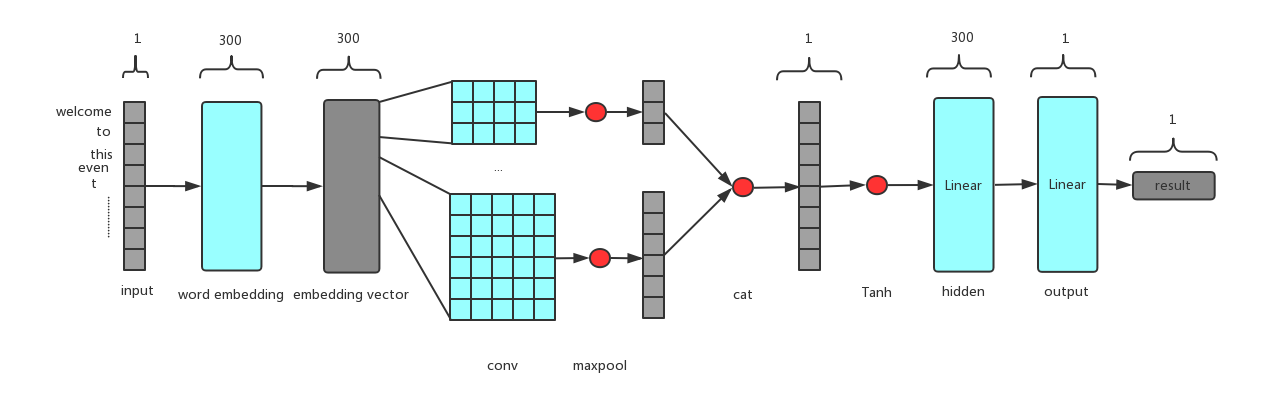
\includegraphics[width=16cm]{conv_ranker.png}
    \caption{带卷积层的神经网络}
    \captionsetup{font=footnotesize,margin=30pt}\caption*{图中灰色的方块表示向量,蓝色的表示网络,红色的圆点表示算符。在计算过程中,输入是文本序列,然后首先经过词向量层转换成词向量,然后进行卷积和池化(max-pooling),将结果拼接起来,然后使用双曲正切(tanh)归一话,最后经过一个带隐含层的线性前馈神经网络输出最终结果。}
    \label{f21}
\end{figure} 

\subsection{带GRU的神经网络}
\subsubsection{RNN在自然语言处理中的应用}
RNN在自然语言处理中运用的十分广泛,是因为它克服了卷积层的弊病。卷积层中由于卷积核感受野的限制,在某些情况下不能很好的收集原始文本中的信息。同时由于自然语言的局部相关性有时候不是那么明显,使用卷积层也不能总是达到很好的效果。而RNN则不同,RNN的感受野是整个句子,同时RNN对文本从左到右(或双向阅读)的处理方式也和人阅读文本时十分类似,所以RNN天然适合自然语言处理。

在实际运用中,为了防止文本序列过长而导致的梯度消失的问题,我们通常会使用RNN的变体:LSTM或者GRU。
\subsubsection{网络结构}
在上一小节,本文使用了卷积层对原始输入文本转换成的词向量进行了处理,得到了一个新的特征向量。这个过程也可以看成是定义了一个函数\(f:R^{m\times k}\mapsto R^n\),将原本在\(R^{m\times k}\)空间中的样本编码到了\(R^n\)中。这样做的目的是可以方便后续处理,相当于把一条文本转换成了一个向量,接下来的工作就在这向量上展开了。但如何去找到一个这样的函数\textit{f},则是这种方法成败的关键。本文希望\textit{f}有如下的特点:1)能处理序列信息。2)能在转换过程中尽量保留原始信息。3)易于实现。而本文之前使用的卷积层并不完全满足这三个条件。首先,它能处理序列信息,但它处理序列信息的能力来源于窗口大小的设置,因此,合理的设置窗口大小非常重要。而在文本处理中,如何设置窗口大小是件困难的事情。其次,因为池化层的存在,它在转换过程中能保留多少原始信息是存疑的。

而另一种处理时序信息的网络结构循环神经网络,则可以很好的满足上面三个条件。所以近年来这种网络也在自然语言处理上得到了广泛的应用,例如在序列到序列模型中,循环神经网络就常常被用在编码/解码环节。同样在这里,本文使用循环神经网络的一种形式$\mathrm{GRU}$\cite{DBLP:journals/corr/ChungGCB14}作为编码器。

\paragraph{GRU}
GRU(gated recurrent network,图\ref{f22})是为了克服传统的循环神经网络中无法很好的处理远距离依赖而提出的$\mathrm{LSTM}$的一个变体。它相较于$\mathrm{LSTM}$来说更加简单,但仍保持着不错的效果\cite{DBLP:journals/corr/ChungGCB14}。GRU的前向传播如公式(\ref{3-9}),公式(\ref{3-10}),公式(\ref{3-11})。其中,\textit{W,U,b}都是参数。\(x_t\)为输入向量,\(h_t\)为输出向量,\(z_t,r_t\)为更新门和重置门向量。同样的,根据链式法则,可以得到其反向传播公式。

\begin{figure}[htb]
    \centering
    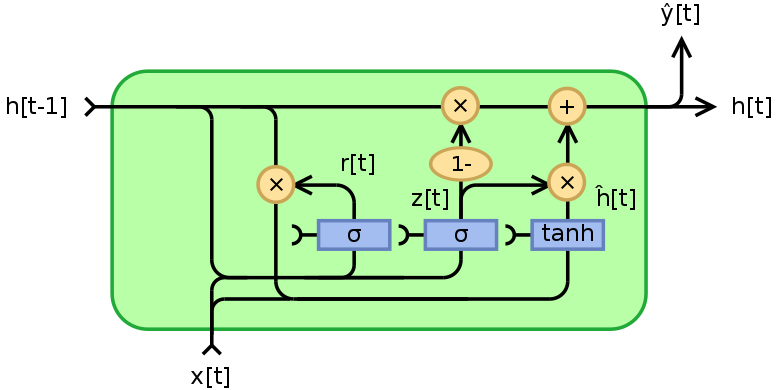
\includegraphics[width=11.5cm]{GRU.png}
    \caption{GRU}
    \captionsetup{font=footnotesize,margin=30pt}\caption*{图中\(z[t]\)为更新门,\(r[t]\)为重置门。\(h[t]\)为当前\textit{t}时刻的隐含状态,橙色的圆点为算符,蓝色方框为某非线性函数}
    \label{f22}
\end{figure}

\begin{equation}\label{3-9}
z_t=\sigma_z(W_zx_t+U_zh_{t-1}+b_z) 
\end{equation}
\begin{equation}\label{3-10}
r_t=\sigma_r(W_rx_t+U_rh_{t-1}+b_r) 
\end{equation}
\begin{equation}\label{3-11}
h_t=(1-z_t)\cdot h_{t-1}+z_t\cdot tanh(W_hx_t+U_h(r_t\cdot h_{t-1})+b_h)
\end{equation}

\paragraph{带GRU的预测器}
将之前的神经网络的卷积层替换成本小节介绍的GRU,本文便得到了另一个新的预测器(如图\ref{f23})。可以看出,该预测器的结构与之前的神经网络十分相似,仅在编码环节有所不同。

\begin{figure}[htb]
    \centering
    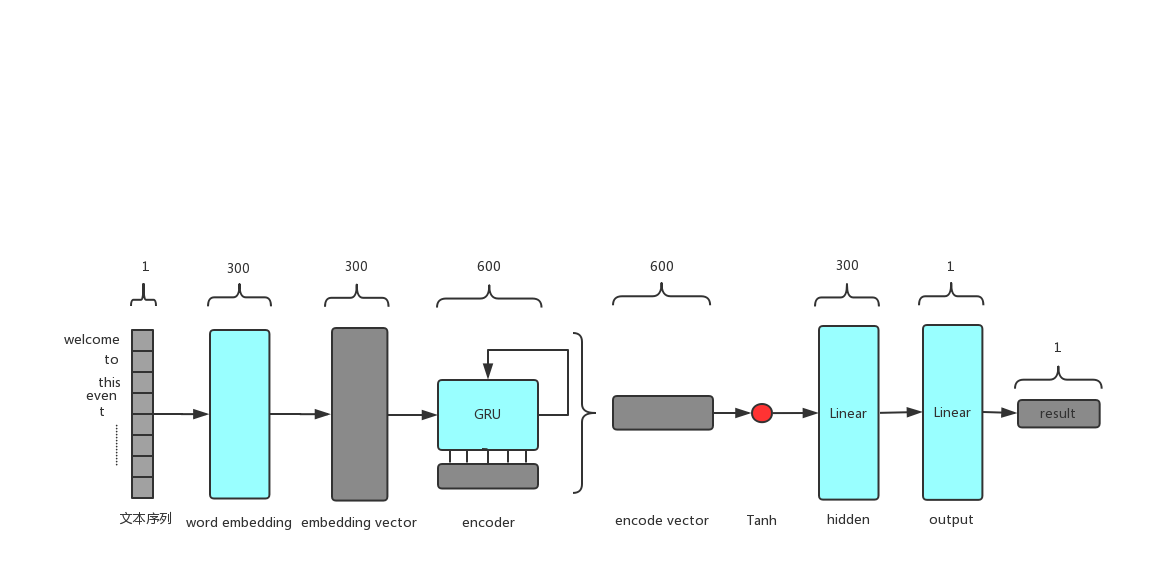
\includegraphics[width=16cm]{gru_ranker.png}
    \caption{带GRU的神经网络}
    \captionsetup{font=footnotesize,margin=30pt}\caption*{图中各色块和圆点的意义同图\ref{f21}。在计算过程中,本文首先将序列转换成词向量,然后使用GRU进行编码,获得一个新的向量(\textit{encode vector}),然后使用双曲正切(\textit{tanh})归一化,最后经过一个带隐含层的线性前馈神经网络输出最终结果。}
    \label{f23}
\end{figure}
\subsection{词向量的初始化}
在自然语言处理中,如何表示词是值得研究的问题。而词向量是指自然语言处理中将词映射到向量的一种方式。在上一章中,本文使用独热编码作为词向量。这种表示方式固然有其简单易实现的特点,但也有维度高,稀疏,词之间相关性差的缺点。因此在本章中,本文使用word2vec\cite{word2vec}算法来计算词向量。

在具体实现中,本文尝试了两种方式来初始化词向量:1)使用gensim中提供的word2vec函数来计算词向量。并使用它来进行初始化。2)使用归一化的服从正态分布的随机数来初始化词向量。实验证明这两种方式并没有显著区别,因此,在实验中,本文采用了第一个方法。
\subsection{实验设计与结果}
在本节中,本文将通过两个实验来比较不同的文本处理方式的效果。在第一个实验中,本文将比较不同的预测器在预测参与人数上的差异:本文首先使用百分之八十的事件训练预测器,并使用剩下的数据对预测器进行评估。在第二个实验中,本文将使用本章提出的预测算法来取代上一章预测事件结果中使用的事件描述评价器,来比较不同的文本处理方式对预测事件结果准确率的提升。
\subsubsection{数据集,评估方式及参数设置}
本次实验所使用的数据集与上一章完全相同。本文所用的数据集来自meetup的LA市,包含超过20万个事件,数据集的详细情况见表\ref{t1-1}。在评估方式上,针对第一个实验,本文使用了均方误差来衡量预测值和参与人数的距离。在第二个实验中,和上一章相同,本文仍使用准确率作为评价指标。在参数设置方面,本文使用了网格搜索和四折交叉验证的方式,确定了最佳参数如表\ref{t2-1}所示。

\begin{table}[htb]
\caption{\label{t2-1}网络参数设置}
\centering
\begin{tabular*}{\linewidth}{p{0.333\linewidth}p{0.333\linewidth}p{0.333\linewidth}}
\toprule
    参数         & 带GRU的神经网络 & 带卷积层的神经网络 \\
\midrule
    词向量维度      & 300       & 300       \\
    GRU的\(h_t\)维度   & 600       & 无         \\
    卷积核窗口大小    & 无         & 1,2,3,4,5 \\
    线性神经网络隐层维度 & 300       & 300      \\ 
\bottomrule
\end{tabular*}
\end{table}

\subsubsection{实验结果与分析}
\paragraph{实验一的结果与分析}
本文使用了百分之八十的事件训练预测器,并使用剩下的数据对预测器进行评估。训练及测试过程的损失函数变化如图\ref{f2-4},其中纵轴为参与人数(对数),横轴为循环次数(×100)。
\begin{figure}[htb]
	\centering
	\begin{subfigure}{.49\textwidth}
		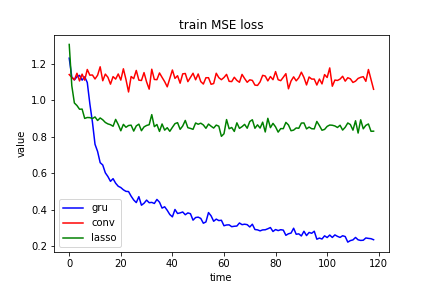
\includegraphics[width=\textwidth]{trainloss.png}
		\caption{train MSE loss}
	\end{subfigure}
%%%%%%%%%%%%%%
	\begin{subfigure}{.49\textwidth}
		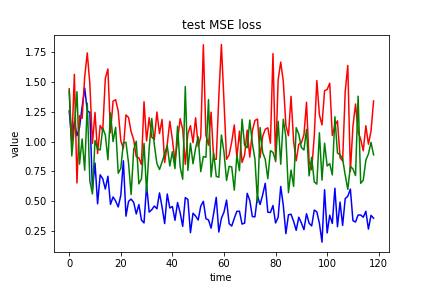
\includegraphics[width=\textwidth]{testloss.png}
		\caption{test MSE loss}
	\end{subfigure}
    \caption{实验结果}
    \label{f2-4}
\end{figure} 
从图中可以看出,使用GRU作为编码器的神经网络的表现最好,其次是线性预测器,使用卷积层的神经网络表现最糟糕。这点是出乎意料的,原因可能是卷积层在自然语言处理中比较适合短文本分类,即能区分文法上有明显区别的句子。但由于其感受野的限制,不适合用来区分整个文本的语义区别。而另一点值得注意的是尽管GRU在此次实验中的表现最好,但是其结果仍然不是特别理想(从测试环节损失函数的曲线的抖动也可以看出这一点)。这是因为在预测过程中本文仅使用了事件描述这一属性,而没有参考其他属性,例如事件种类,所在组别,举办时间,举办地点,举办者等。属性的缺失限制了这些预测器的上限。如果在预测时加上了这些属性,参考第一章,可以预见准确度应该会有所提升。 
\paragraph{实验二的结果与分析}\label{train_discrimiator}
本次实验的数据集和分类算法与第二章所采用的方式完全一致,仅在处理文本时使用本章提出的使用GRU作为编码器的神经网络。本次实验仍使用百分之七十的数据作为训练数据,剩余的百分之三十则用来评估分类结果。本次实验使用交叉验证和网格搜索的方式来确定最佳参数,实验结果见表\ref{t2-2}。

\begin{table}[htb] 
    \centering
    \caption{\label{t2-2}使用不同文本处理方法和分类器对预测事件结果的影响}
    \begin{tabular*}{\linewidth}{p{0.2\linewidth}p{0.2\linewidth}p{0.25\linewidth}p{0.25\linewidth}}
\toprule 
分类器&不包含事件描述&使用拉索回归处理文本&使用GRU神经网络处理文本\\
\midrule
Adaboost & 0.762 & 0.791 & 0.801 \\
Decision Tree& 0.763 & 0.786 & 0.811\\
Knn & 0.764 & 0.782 & 0.799 \\
Random Forest & 0.762 & 0.788 & \textbf{0.830} \\
\bottomrule
    \end{tabular*}
\end{table}

实验结果可以看出,使用$\mathrm{GRU}$作为编码器的神经网络来处理事件描述的准确率最高,其次是使用拉索回归处理。排除事件描述作为分类属性的结果最差。所以,在使用了新的文本处理方式后,预测事件成功率的准确度有所提高。这反过来也证明了事件描述在事件成功/事件参与人数上的重要作用。
\subsection{本章小结}
本章主要研究了不同的事件描述处理方式对预测事件结果和事件参与度的影响。实验证明,使用GRU的神经网络无论在预测事件参与人数的精度上还是在预测事件结果上都要高于其他两个预测器。这也证明了循环神经网络在处理时序信息上的能力。

与此同时,我们还可以看到,光凭事件描述是无法很准确的预测事件参与人数的。因为哪怕是排除了事件描述,事件其他属性的随机效应的确定系数也达到了0.494。这说明了其他属性在决定事件参与度上也是很重要的,而如果缺失了这一部分信息,自然无法准确的预测出事件参与人数来。

在下一章,本文将提出一个带变分编码器的端到端的网络作为事件描述生成模型,使用本章的带GRU的神经网络作为判别模型。这两个神经网络将被运用在一个生成对抗网络中,以训练出可以生成新的事件描述的网络模型。
% \end{document} 